\titre{}
\theme{derivation}
\auteur{Nathan Scheinmann}
\niveau{3M}
\source{sesamath3e}
\type{serie}
\piments{2}
\pts{}
\annee{2425}

\contenu{
\tcblower
On dispose de 288 mètres de clôture grillagée pour construire 6 enclos pour un zoo le plan ci-contre :

\begin{center}
	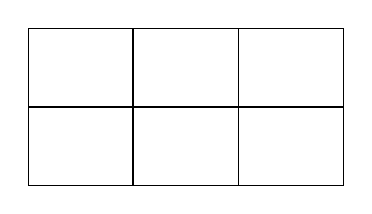
\begin{tikzpicture}
\draw (0,0) rectangle (4,2);
\draw (1.33,0) -- (1.33,2);
\draw (2.67,0) -- (2.67,2);
\draw (0,1) -- (4,1);
\end{tikzpicture}
\end{center}

Quelles dimensions donner à ces enclos de manière à maximiser leur surface au sol ?
}
\correction{
\tcblower
\textit{Generated by AI}

D'après le plan, les 6 enclos sont disposés en 2 rangées de 3 enclos chacune.

Notons :
\begin{itemize}
\item $x$ : la largeur de chaque enclos (dimension horizontale)
\item $y$ : la longueur de chaque enclos (dimension verticale)
\end{itemize}

\textbf{Contrainte de la clôture :}

En comptant toutes les portions de clôture nécessaires :
\begin{itemize}
\item Côtés horizontaux : $2 \times 3x = 6x$ (haut) $+ 6x$ (bas) $= 12x$
\item Côtés verticaux intérieurs (séparations verticales) : $4 \times y = 4y$ (4 séparations verticales)
\item Côtés horizontaux intérieurs (séparation horizontale centrale) : $3x$ (1 séparation horizontale)
\item Côtés verticaux extérieurs : $2y$ (gauche) $+ 2y$ (droite) $= 4y$
\end{itemize}

Non, reprenons plus clairement. Il y a :
\begin{itemize}
\item 2 côtés horizontaux de longueur $3x$ (haut et bas) : $2 \times 3x = 6x$
\item 4 côtés verticaux extérieurs de longueur $y$ (2 à gauche, 2 à droite... non, 2 de chaque côté) : $2 \times 2y = 4y$
\item 4 séparations verticales intérieures de longueur $y$ : $4y$
\item 1 séparation horizontale de longueur $3x$ : $3x$
\end{itemize}

Total : $6x + 4y + 4y + 3x = 9x + 8y = 288$

\textbf{Surface totale :}

L'aire totale est :
\[
\mathcal{A} = 3x \times 2y = 6xy
\]

De la contrainte $9x + 8y = 288$, on tire :
\[
y = \frac{288 - 9x}{8}
\]

Donc :
\[
\mathcal{A}(x) = 6x \cdot \frac{288 - 9x}{8} = \frac{6x(288 - 9x)}{8} = \frac{3x(288 - 9x)}{4} = \frac{864x - 27x^2}{4}
\]

\textbf{Maximisation :}

\[
\mathcal{A}'(x) = \frac{864 - 54x}{4} = \frac{54(16 - x)}{4}
\]

$\mathcal{A}'(x) = 0 \Leftrightarrow x = 16$

Pour $x = 16$ :
\[
y = \frac{288 - 9 \times 16}{8} = \frac{288 - 144}{8} = \frac{144}{8} = 18
\]

\textbf{Réponse :} Chaque enclos doit mesurer $16~\text{m}$ de largeur et $18~\text{m}$ de longueur pour une surface totale maximale de $\mathcal{A} = 6 \times 16 \times 18 = 1728~\text{m}^2$.
}

